\documentclass{article}
\PassOptionsToPackage{numbers,compress}{natbib}
\usepackage[dblblindworkshop,final]{neurips_2026}
\usepackage[utf8]{inputenc}
\usepackage[T1]{fontenc}
\usepackage{hyperref}
\usepackage{url}
\usepackage{booktabs}
\usepackage{amsmath}
\usepackage{microtype}
\usepackage{xcolor}
\usepackage{graphicx}
\usepackage{enumitem}

\title{Do Simulated Users Reveal Behaviorally Observable States During Human--LLM Joint Decision Making?}
\workshoptitle{SocialAgent: Second Workshop on Generative Agents and Simulations for Social Science}
\author{
\normalfont
Yinqi Huang$^{1}$ \quad Ruohan Feng$^{1}$ \quad Yilin Cai$^{1}$\\
Mei Li$^{2}$ \quad Vineet Upadhya$^{1}$ \quad Robert Wilson$^{1}$\\[0.5em]
$^{1}$Georgia Institute of Technology\\
$^{2}$Guangzhou Women and Children's Medical Center\\
\texttt{yhuang994@gatech.edu}
}
\hypersetup{pdftitle={Do Simulated Users Reveal Behaviorally Observable States During Human--LLM Joint Decision Making?},pdfauthor={Yinqi Huang; Ruohan Feng; Yilin Cai; Mei Li; Vineet Upadhya; Robert Wilson}}
\newcommand{\R}{\mathit{R}}
\newcommand{\I}{\mathit{I}}
\newcommand{\A}{\mathit{A}}
\newcommand{\U}{\mathit{U}}

\begin{document}
\maketitle

\begin{abstract}
Simulated users can produce plausible dialogue and numerical state reports without those reports necessarily structuring behavior. We evaluate behavioral observability in a controlled persona-agent sandbox spanning medical, legal, and finance decisions. For self-reported urgency, information need, intended action, and uncertainty, we compare out-of-persona prediction from known experimental context with prediction from context plus observable interaction. AI advice selectively changes reported states, but responsiveness and behavioral observability diverge. Information need has the clearest incremental behavioral footprint; uncertainty has a weak additional signal, while urgency and intended action add little after context is known. The information-need pattern remains when text is removed and is directionally consistent across all three domains, indicating that structured search and evidence acquisition carry much of the signal. A complementary transition analysis shows that simulated users follow AI advice more strongly than they move toward the fixed task reference. An interim matched human study provides descriptive comparisons of AI-related state changes, decisions, and evidence acquisition. The AI-confidence--information-need association varies by recommendation level in the analyzed subset, while formal human behavioral-observability and transfer tests remain pending. Persona simulation can therefore generate falsifiable state--behavior hypotheses and identify measurement requirements; matched human interaction determines which relationships transfer.
\end{abstract}


\section{Why test observability before recruiting people?}


LLM-based agents are increasingly used to simulate individuals, populations, and interactive social worlds \citep{aher2023using,park2023generative,argyle2023out,horton2023homo,li2026matraix}. Their scale creates a tempting inference: if an agent produces realistic language, stable personas, and sensible state ratings, then its trajectory can stand in for human behavior. Existing evidence makes that inference unsafe. Synthetic responses can recover aggregate patterns while changing variation and coefficient structure \citep{bisbee2024synthetic}; simulated populations may flatten identity groups \citep{wang2025flatten}; and proposals to use models as participants emphasize task- and stage-specific validity rather than general replacement \citep{dillion2023replace}.

Experimental records capture only the behaviors that a study is designed to measure. Once recruitment begins, unrecorded behavior cannot be recovered through analysis \citep{huang2026projection}. A pre-human simulation is therefore useful not because it supplies human evidence, but because it can expose which state probes, information actions, and event channels must be recorded before the human protocol fixes that information bottleneck.

\begin{figure}[t]
  \centering
  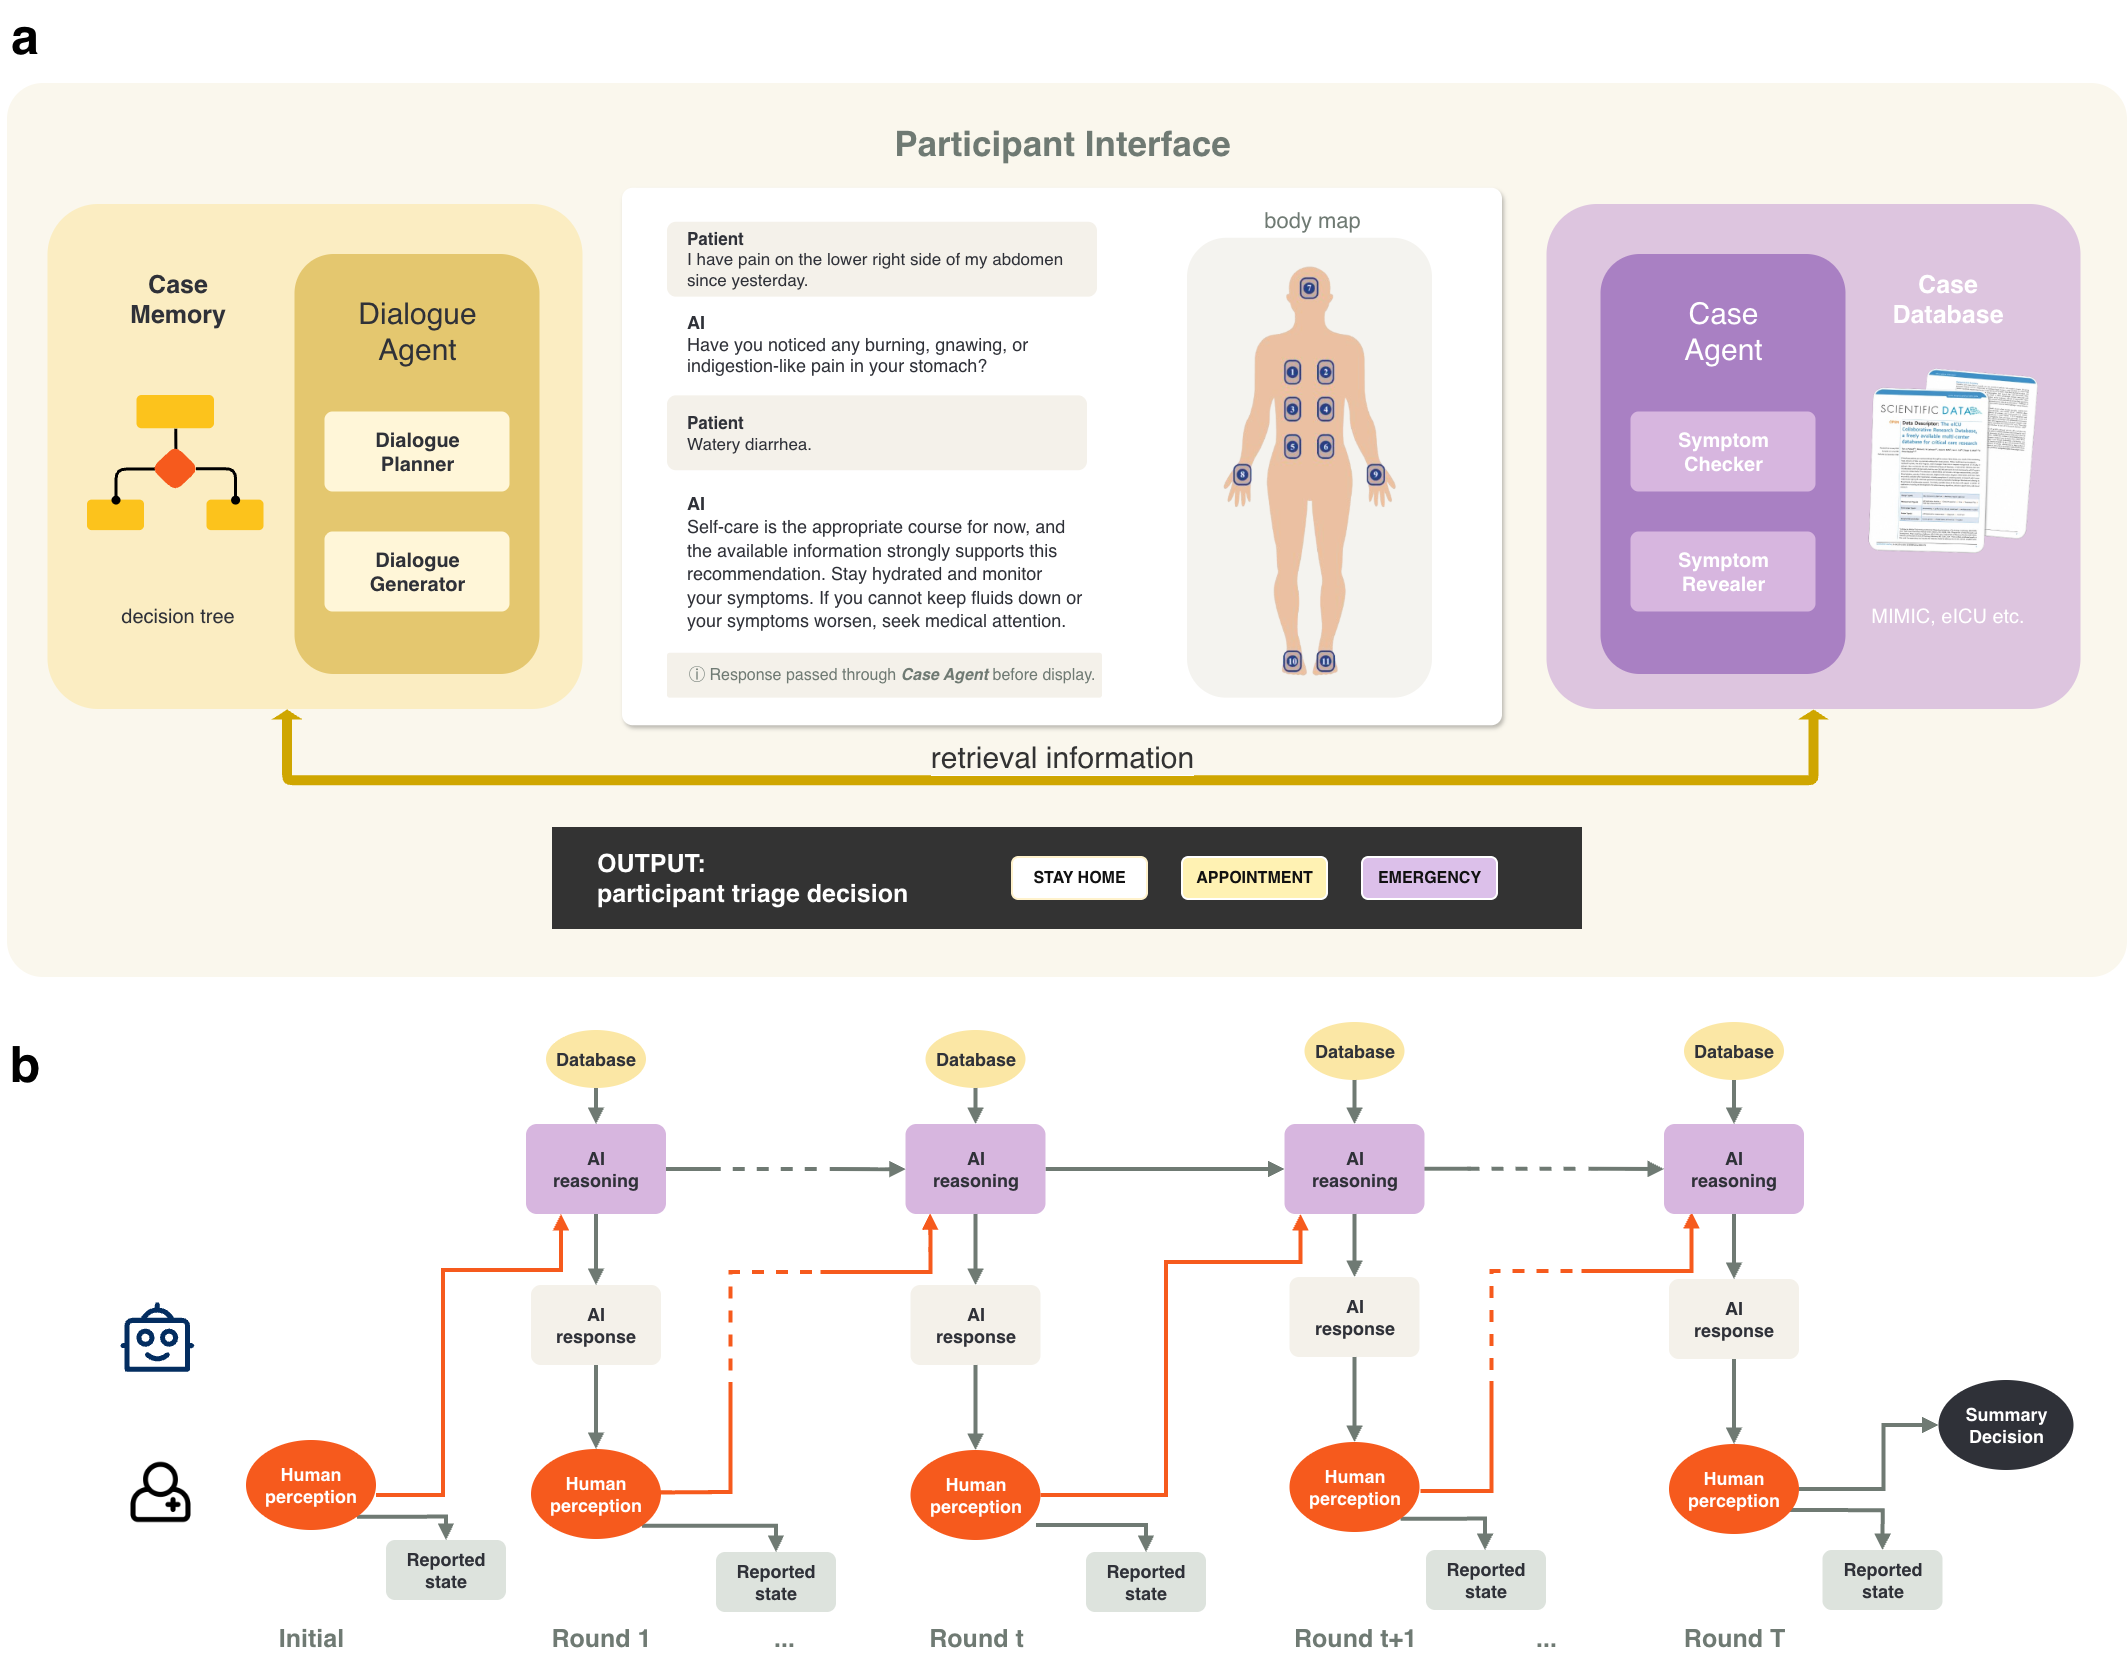
\includegraphics[width=\linewidth]{figs/task.png}
  \caption{\textbf{
  Overview of the medical self-triage task.}
  \textbf{(a)} LLM interface for human participants. A dialogue agent maintains case memory and conducts a symptom-focused interaction. A body map supports localization, while a case agent reveals information from structured case definitions. The broader critical-care data framework draws on MIMIC-III and eICU; the analyzed cases are not direct samples from either database. Participants integrate the accumulated evidence and report a triage decision ranging from staying home to seeking emergency care.
  \textbf{(b)} Sequential human-LLM interaction in one conversation. At each round, case information from the dataset informs AI reasoning and the resulting AI response, which is then interpreted by the participant. The participant's perception contributes to an updated reported state and can influence subsequent AI reasoning, forming a closed-loop interaction that repeats through Round $T$. The sequence terminates with a summary triage decision.
  }
  \label{fig:task}
\end{figure}


The distinction is consequential in interactive decisions. A simulator can readily generate a numerical rating when asked; the scientific question is whether that report is reflected in what the simulated user subsequently does. We define the self-reported state as $X_t=[\R_t,\I_t,\A_t,\U_t]$: perceived risk or urgency, information need, intended action, and uncertainty, where $\U_t=100-\text{confidence}_t$. Experimental context $C_t$ comprises case, domain, turn, recommendation level, and AI confidence. Observable interaction $Y_t$ comprises the logged language, search, evidence, timing, and stopping behavior. Thus $X_t$ is withheld from the estimator, $C_t$ is known by design, and $Y_t$ is recoverable from the interaction log (Fig.~\ref{fig:framework}). Behavioral observability tests state--behavior correspondence; it does not treat a self-report as a transformer's neural representation.

This criterion matters especially for consequential human--LLM interaction. Medical symptom checkers remain variable in diagnostic and triage accuracy \citep{wallace2022symptom}; uncertainty communication is itself part of safe decision support \citep{kompa2021uncertainty}; and a large randomized study found that strong stand-alone model performance did not translate into equally strong public use of the same models \citep{bean2026reliability}. AI advice can also alter human judgments over repeated interaction \citep{glickman2025feedback}, so advice following, reported confidence, search, and task-reference alignment should not be collapsed into a single performance score. Governance concerns may arise from informational influence before a system has formal clinical authority \citep{huang2026clinical}; understanding the behavioral pathway is therefore an empirical as well as a regulatory problem.

We make three contributions. First, we operationalize behavioral observability as the incremental out-of-persona prediction gained by adding interaction behavior to known context. Second, a crossed pre-human simulation separates three claims often treated as equivalent: a report can be \emph{responsive} to advice, \emph{predictable} from context, or additionally \emph{expressed} in behavior. Third, we carry the same cases, state scales, turn unit, and evidence representation into a matched human study designed to test transfer; the present human analyses are descriptive. The central finding is selective: information need has the clearest behavioral footprint, whereas intended action changes strongly with advice but contributes almost no residual behavioral signal after context is known.

Figure~\ref{fig:task} summarizes the interaction cycle shared by simulated users and human participants. Figure~\ref{fig:framework} presents a closed-loop model that explicitly distinguishes reported state, known experimental context, and observable behavior.

\begin{figure}[t]
\centering
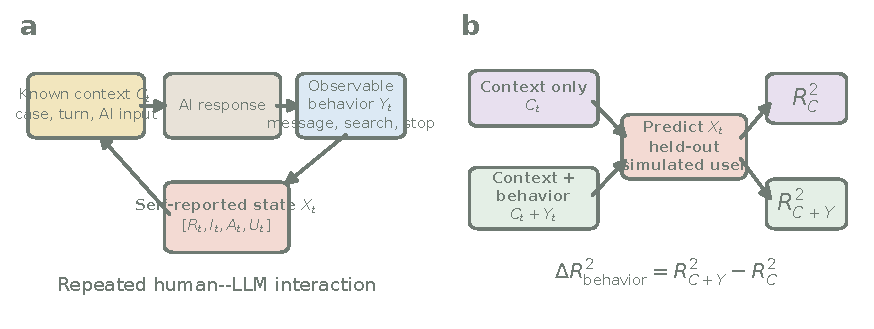
\includegraphics[width=\linewidth]{figs/flowchart.pdf}
\caption{\textbf{Closed-loop human--LLM interaction and behavioral observability framework.}
\textbf{(a)} Known context $C_t$ and AI output shape a participant's self-reported state $X_t=[R_t,I_t,A_t,U_t]$ and observable behavior $Y_t$ over repeated interaction.
\textbf{(b)} Behavioral observability predicts the same reported state from context alone or from context plus observable behavior. The incremental information carried by behavior is
$\Delta R^2 = R^2_{\mathrm{context+behavior}} - R^2_{\mathrm{context}}$.
A positive $\Delta R^2$ means that interaction behavior improves prediction of the reported state beyond experimental context.}
\label{fig:framework}
\end{figure}
\section{A sandbox for falsifiable state--behavior hypotheses}
\subsection{Comparable decisions across three domains}

We instantiated the framework using the MatrAIx Persona-8B persona infrastructure \citep{li2026matraix}, with GPT-4.1-mini as the persona-agent backbone. Four personas completed 30 fixed cases: ten each in medical triage, legal summons response, and finance dispute response, with five lower- and five higher-reference cases per domain. Every case followed the same abstract sequence: initial uncertainty, information acquisition, state update, continue/stop, and final action. The medical task used the human study's canonical evidence definitions. Its broader critical-care data framework draws on resources including MIMIC-III and eICU \citep{johnson2016mimic,pollard2018eicu}; the analyzed cases are not direct samples from either database. Legal and finance tasks were constructed from public OATH and CFPB sources and relevant regulatory guidance \citep{oathdata2026,cfpb2026,rege2026}.

The cross-domain design tests whether the measurement framework produces similar state--behavior relationships across distinct decisions. Each case provides initial and revealable evidence, selectable information clusters, conversation, stopping, and a final 0--100 action judgment. Medical action runs from self-care to calling an ambulance; legal and finance cases use analogous lower--higher escalation scales. A canonical evidence ID is the unit of information acquired through either a structured reveal or an explicit case-consistent conversational disclosure. This separates information-seeking actions from information obtained.

\subsection{Advice perturbations and private probes}

Every persona encountered each case under a $2\times2$ advice condition: lower versus higher AI recommendation escalation (the formal factor \emph{Direction}) and low versus high AI \emph{Confidence}. Substantive interpretation was held fixed within a case state; deterministic policy sentences varied only the assigned recommendation level and stated confidence. Recommendation escalation targeted intended action, whereas AI confidence targeted reported uncertainty and information need.

After the initial case and each completed interaction cycle, a separate stateless call to the same persona-agent backbone, initialized with the same persona prompt, requested integer ratings from 0--100 for perceived urgency, information needed, intended action, and uncertainty. The call received the opening problem and visible dialogue through that turn. Its self-reports were stored outside the dialogue, were not appended to subsequent persona context, and were unavailable to the advising model and behavioral estimator. Current-turn behavioral features preceded the corresponding post-turn report; neither probe values nor future interaction entered prediction features. Turn 0 denotes the pre-assistance baseline; turn 1 onward denotes a complete information/reasoning cycle rather than a click.

Because the evaluator observes the dialogue history, its reports may partly reflect the same interaction information used by the behavioral predictor; we therefore interpret observability as predictive correspondence with elicited reports rather than independent validation of latent internal states.

The balanced design yielded 480 trials and 2,362 aligned post-turn observations. Each persona contributed 120 trials, so case and policy balance cannot masquerade as persona variation. The grouping unit for all prediction was persona, not turn. Four personas provide broad case stress testing but not stable estimates of persona moderators; the experiment targets state--behavior mappings rather than a population distribution of simulated traits.


\subsection{Behavioral observability beyond context}

For each state separately, a regularized linear model predicted the current self-report under four-fold grouped-by-persona cross-validation; there is no single multivariate $R^2$ over all four states. Model 1, $X_t\leftarrow C_t$, asks how well case, domain, turn, recommendation escalation, and AI confidence predict the report without observing behavior. Model 2, $X_t\leftarrow C_t+Y_t$, adds behavioral features defined in the supplement. Neither current nor previous self-reports entered the estimator. We define
\[
\Delta R^2_{\mathrm{behavior}}=R^2_{\mathrm{context+behavior}}-R^2_{\mathrm{context-only}}.
\]
$R^2$ measures out-of-persona predictive performance for a self-reported state; $\Delta R^2_{\mathrm{behavior}}$ measures the additional predictive information contributed by observable behavior after context is known. High total $R^2$ and high behavioral observability are different quantities. Intended action can be highly predictable because case identity and AI recommendation escalation already constrain it even when behavior adds almost nothing. Information need can be less predictable overall while search and evidence behavior add substantially more beyond context. We therefore distinguish \emph{predictability} (can the report be predicted?), \emph{behavioral observability} (does behavior add beyond context?), and \emph{transferability} (does the same relation occur in humans?).

We complement incremental prediction with manipulation contrasts, modality ablations, controlled trace corruption, domain-specific estimates, and a turn-level transition analysis. The latter describes conditional updating of reported state and action given pre-turn state, advice, evidence, and task target. It is not used to identify a utility function or a causal mediation pathway. Full feature definitions, seeds, case construction, and robustness procedures appear in Appendix~\ref{app:supplement}.


\section{Five results that demonstrate the simulator's scope}
\begin{figure}[t]
  \centering
  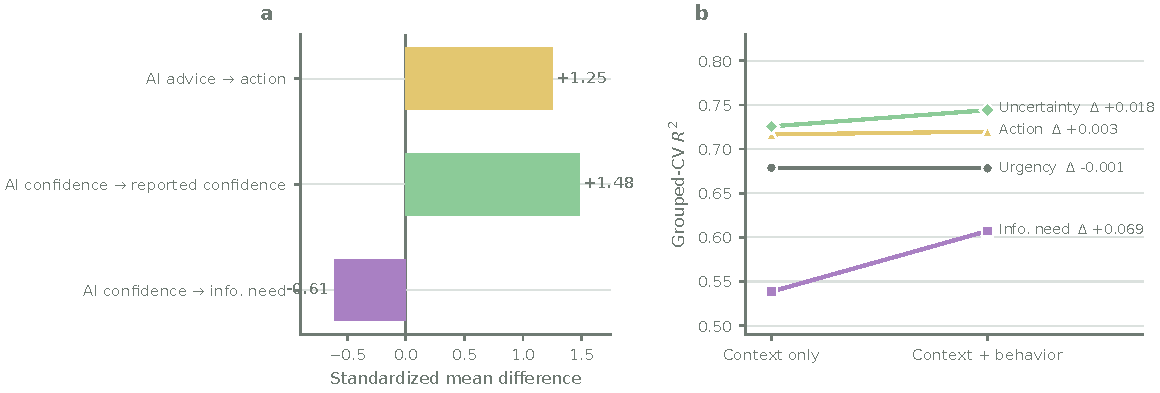
\includegraphics[width=0.94\linewidth]{figs/main_results.pdf}
  \caption{Selective responsiveness and behavioral observability. (a) Standardized final-state shifts from the crossed advice manipulation. (b) For each state, connected points show grouped-by-persona prediction from context alone and after adding observable behavior. The vertical change is $\Delta R^2_{\mathrm{behavior}}$; information need shows the largest positive increment.}
  \label{fig:results}
\end{figure}


\subsection{AI advice selectively changes reported state}

The perturbations produced differentiated final-state shifts (Fig.~\ref{fig:results}a). Higher AI recommendations increased final intended action by 1.25 standardized mean differences. High AI confidence increased reported confidence by 1.48 and reduced information need by $0.61$ standardized mean differences. These differentiated reports establish responsiveness; behavioral observability requires a separate test.

A simulated user can map a higher recommendation to a higher action rating while leaving search and stopping unchanged. Conversely, a state can organize search even when its final manipulation contrast is modest. The next analysis therefore conditions on the inputs that produced these shifts.


\subsection{Reported states can be predictable from context}

Information need showed the clearest incremental behavioral signal (Fig.~\ref{fig:results}b). Context alone predicted urgency ($R^2=.679$), information need (.539), intended action (.717), and uncertainty (.726). Adding behavior changed these values to .678, .607, .720, and .744, respectively. Intended action was highly predictable because case and AI advice already constrained it, but behavior added only .003. Urgency added approximately no information ($-.001$), and uncertainty increased by .018.

Information need added $\Delta R^2=.069$. It was not the best-predicted rating overall; observing behavior added the most beyond knowing the experimental context. This is the principal simulation finding: responsiveness, predictability, and behavioral observability are distinct properties.

The practical consequence is state-specific measurement. Information need is the strongest candidate for partial passive inference from interaction logs. Its self-report remains part of the human transfer test, and the other states retain direct measurement unless human data establish stronger observability.

\subsection{Information need is reflected in search and evidence acquisition}

Feature ablations located the information-need signal in interaction structure. Removing text left context-plus-behavior prediction at $R^2=.604$, close to the full model's .607, and the evidence trajectory alone reached .574. Search, accumulated evidence, and continuation carried more of the footprint than self-description. Text alone was less informative, and sparse continue/stop logs preserved only a coarse trace. Uncertainty required a broader combination of channels and retained a smaller increment.

Turn number is included in the context-only baseline, but accumulated and remaining evidence measure within-case progress more precisely than turn alone. Part of the information-need increment may therefore reflect progression through the available evidence rather than a distinct search strategy. The result establishes incremental prediction from observable interaction; it does not decompose task progress from active information seeking or identify a causal effect of search on information need.

Controlled corruption reduced reconstruction when behavioral events or structured information actions were removed, while known context preserved the portion already determined by case and manipulation. This stress test identifies canonical reveal IDs, action timing, and stopping as essential human-study measurements.

\subsection{The mapping is directionally consistent across domains}

\begin{figure}[t]
  \centering
  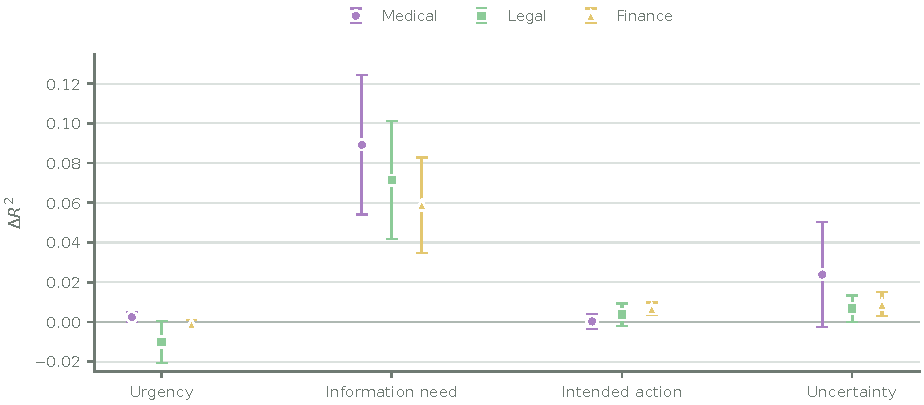
\includegraphics[width=0.70\linewidth]{figs/domain_specific_incremental_observability.pdf}
  \caption{Domain-specific behavioral observability. Points and persona-bootstrap standard errors show $\Delta R^2$ for each self-reported state in medical, legal, and finance decisions. The zero line marks no incremental behavioral information.}
  \label{fig:domain-observability}
\end{figure}


All three domains used the same task architecture and advice manipulation. Because the pooled model includes domain in $C_t$, its increment asks whether behavior contains information beyond domain, case, turn, and AI condition. Within-domain models ask whether the same incremental relation appears in each domain. The information-need increment was positive in medicine (.089), law (.071), and finance (.059; Fig.~\ref{fig:domain-observability}), showing directional consistency with varying magnitude.

Across simulated users, information need was the only self-reported state with a clear incremental behavioral footprint in all three domains. Search and evidence behavior added information beyond case and AI condition, whereas urgency and intended action added essentially none and uncertainty added little. Variation in magnitude also shows why a single realism score would obscure state- and domain-specific validity.

\subsection{Advice following is not movement toward the task reference}

The observability analysis asks whether $Y_t$ contains information about $X_t$; the transition analysis asks how AI inputs and prior state relate to $X_t\rightarrow X_{t+1}$ updating. Higher AI recommendations predicted upward intended-action updating ($\beta=.510$). High AI confidence predicted reduced information need ($\beta=-.316$) and uncertainty ($\beta=-.855$). The same simulated users moved toward the AI-advised endpoint ($\beta=-.317$ for higher recommendations on AI-target distance), whereas movement toward the fixed task reference was small ($\beta=-.048$).

Advice responsiveness and task-reference improvement measure different properties: discordant advice can shift action away from the case endpoint. Simulated-user evaluation should therefore report advice susceptibility and task-reference convergence separately, especially when informational influence matters without formal clinical authority \citep{huang2026clinical}.

\section{Preliminary human comparison under matched medical vignettes}
\subsection{A parallel human study}

We analyzed data from 109 human participants who completed the matched medical protocol. The study was conducted under Georgia Institute of Technology IRB protocol IRB2025-388, and all participants provided informed consent. Qualtrics randomized participants to the AI-assisted or human-reasoning condition. Within AI-assisted sessions, recommendation level and AI-confidence cells were balanced at session creation and fixed before interaction. Every returned assistant response began with the assigned recommendation statement, so observed exposure additionally required a participant message and a delivered response. The 218 completed case trajectories contained 184 baseline and 757 post-turn self-reports; 159 trajectories included at least one post-turn report. Eighty-two trajectories received at least one recommendation-bearing assistant response, whereas 136 did not. Recommendation comparisons condition on delivered exposure rather than randomized assistance assignment and are interpreted descriptively; because exposure required dialogue engagement, these subgroup comparisons may reflect selection.

Humans completed fewer mean turns than simulated users for appendicitis (3.42 vs. 5.06) and viral gastroenteritis (4.03 vs. 5.88). Their decisions differed most in appendicitis: mean final action was 48.62 for humans versus 90.63 for simulated users, and reference-action alignment was .202 versus 1.00. Viral-gastroenteritis judgments were closer: final action averaged 24.77 versus 41.25, and alignment was .606 versus .625. The shared protocol therefore produced comparable observables alongside different absolute decisions and reference alignment.

The planned human transfer test mirrors the agent decomposition: $X_{t,\mathrm{human}}$ is a self-reported state, $C_{t,\mathrm{human}}$ is known context, and $Y_{t,\mathrm{human}}$ is logged behavior. Its primary statistic asks whether behavior predicts human information need beyond context, $\Delta R^2_{I,\mathrm{human}}=R^2_{C+Y}-R^2_C>0$. That formal behavioral-observability test remains pending; the results below compare AI effects, actions, and evidence acquisition descriptively. We distinguish agreement in effect direction, effect magnitude, and behavioral channels. Agreement in direction alone does not establish that simulated users and humans express the same state--behavior relationship.

Figure~\ref{fig:human-pilot} plots human and simulated trajectories through turn 6; later ratings remain in the analysis tables. Human standard errors use the observations available at each turn, so later points summarize participants who continued.

\begin{figure}[t]
  \centering
  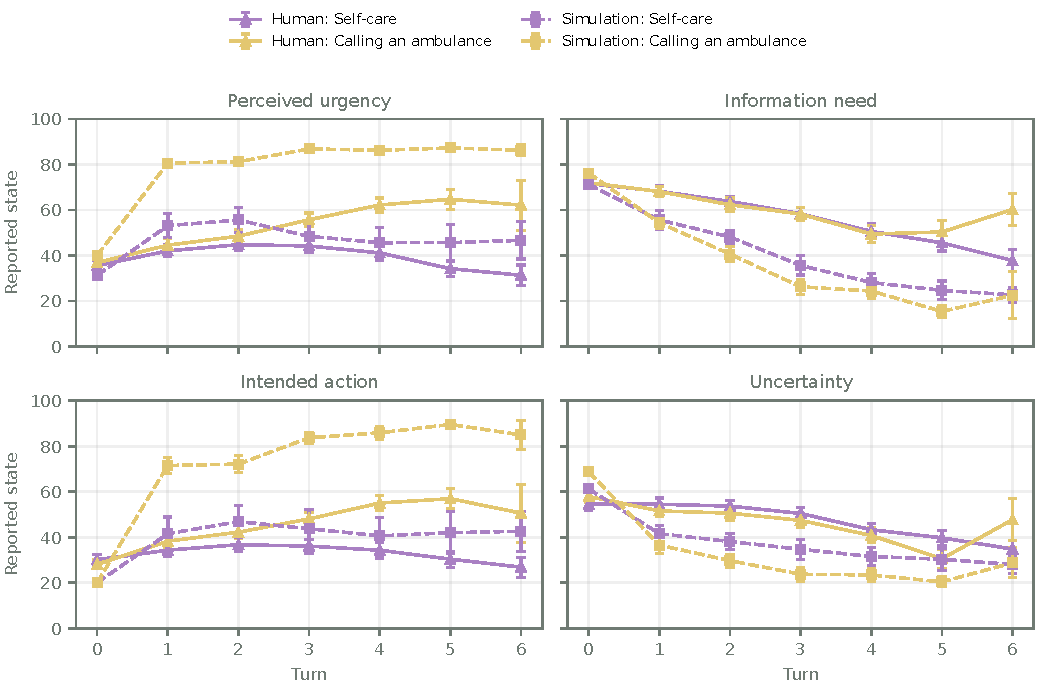
\includegraphics[width=\linewidth]{figs/human_simulation_pilot_trajectories.pdf}
  \caption{Human and simulated medical state trajectories. Solid triangles show human means and SEM; dashed squares show simulated-user means and SEM. Cases are labeled by fixed study reference (Self-care; Calling an ambulance). The baseline contains 92 reports per case; 159, 147, and 142 trajectories contribute at turns 1--3, respectively. At turn 6, 35 Self-care and eight Ambulance trajectories remain. Later human ratings remain in the analysis. Simulated curves contain 16 trials per case nested in four personas.}
  \label{fig:human-pilot}
\end{figure}

\subsection{AI confidence--information need varies by recommendation level}

Among the 82 recommendation-exposed trajectories, the viral case provides the complete case-matched $2\times2$ comparison: 46 human trajectories (cell counts 14, 11, 12, and 9) and 16 simulated trajectories (four personas per cell). The high-minus-low marginal difference in last-minus-first information need was $-6.98$ points in humans and $-20.0$ in simulated users. By recommendation level, the human and simulated contrasts were $-18.81$ and $-25.0$ under lower recommendations, but $+4.86$ and $-15.0$ under higher recommendations. The descriptive association therefore depended on recommendation level and does not establish transfer of the simulated relationship.

The marginal higher-versus-lower recommendation contrast in final action was similar across sources: $+49.52$ points in humans and $+52.50$ in simulated users. Condition-specific patterns were less uniform: the human difference-in-differences was 38.33 points across cells containing 9--14 trajectories. Figure~\ref{fig:human-cells} displays the cell means and SEM. Similar marginal shifts do not imply similar absolute decisions or case-specific reference alignment, which differed across sources, especially for appendicitis.

\begin{table}[t]
  \centering
  \scriptsize
  \caption{Formal Direction $\times$ Confidence cell means for the viral-gastroenteritis case. $\Delta I$ is last-minus-first information need.}
  \label{tab:human-cells}
  \begin{tabular}{@{}llrrrrrr@{}}
    \toprule
    Direction & Confidence & Human $n$ & Human $A$ & Agent $A$ & Human $\Delta I$ & Agent $\Delta I$ & Human turns \\
    \midrule
    Lower  & Low  & 14 & 7.1 & 20 & $-41.6$ & $-30.0$ & 4.9 \\
    Lower  & High & 11 & 9.1 & 10 & $-60.5$ & $-55.0$ & 5.9 \\
    Higher & Low  & 12 & 37.5 & 45 & $-21.4$ & $-42.5$ & 5.8 \\
    Higher & High & 9 & 77.8 & 90 & $-16.6$ & $-57.5$ & 6.7 \\
    \bottomrule
  \end{tabular}
\end{table}

\begin{figure}[t]
  \centering
  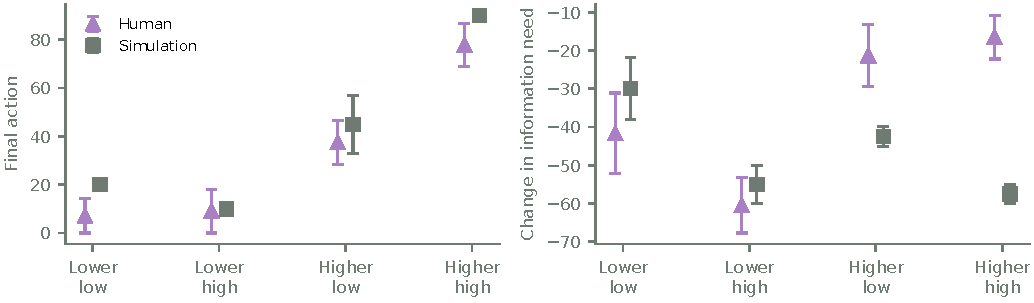
\includegraphics[width=0.84\linewidth]{figs/human_simulation_condition_comparison.pdf}
  \caption{Case-matched viral-gastroenteritis factorial comparison. Points and SEM bars show 46 recommendation-exposed human trajectories (9--14 per cell) and 16 simulated trials (four personas per cell). Cells are categorical and unconnected.}
  \label{fig:human-cells}
\end{figure}

\subsection{Similar search quantities can arise through different channels}

Across all 82 recommendation-exposed human trajectories, logs contained 432 participant messages (5,550 words), 432 assistant responses (17,250 words), 297 conversationally disclosed evidence IDs, and 587 structured evidence IDs. In the 46-trajectory viral subset, humans averaged 12.59 words per message versus 23.47 for simulated users, 4.98 information actions versus 4.63, and 8.80 acquired evidence items versus 7.63. Structured search was similar in scale, while message form differed (Fig.~\ref{fig:human-conversation}).

Both protocols mapped acquired case information to the same canonical evidence IDs and used matched medical-case content and self-report scales. This shared coding makes the number or fraction of acquired evidence items comparable across sources. Humans obtained evidence through dialogue and structured reveal controls, whereas simulated users asked focused questions. Equivalent evidence counts therefore indicate comparable acquired information, not identical information-seeking behavior; the matched analysis keeps the interface-specific action channels separate.

\section{What simulation can and cannot contribute}
\subsection{A stricter validation ladder}

The validation ladder has four stages: advice changes a related self-report; reports vary within interaction; behavior predicts the report beyond context; and the relation transfers under a matched human protocol. The simulation evaluates the first three stages across all four self-reported states, with information need showing the clearest evidence of behavioral observability. Formal transfer to humans remains pending. Intended action passed the responsiveness stage but added almost no behavioral information, whereas information need was both responsive and behaviorally expressed.

This ladder converts ``realism'' from a global impression into discriminating empirical claims. The AI-confidence--information-need comparison depends on recommendation level in the human subset. The marginal recommendation effect on final action is similar across sources, while absolute decisions and task-reference alignment differ. Simulation can therefore guide state and channel measurement without supplying human effect sizes; formal human behavioral-observability analysis determines whether the proposed mapping transfers.

\subsection{Measurement alignment is not source equivalence}

Canonical evidence IDs, explicit information actions, a common turn unit, and identical self-report scales make source-specific models comparable. Simulation observations are nested within four personas and deterministic case policies; human observations are nested within participants, stopping choices, delivered exposure, and interface affordances. Comparisons must therefore account for the different sampling structures and interaction interfaces.

The relevant target is relation-level transfer. For information need, the prospective claim is that behavior adds predictive information beyond context in each source. Advice effects ask whether recommendation level and AI confidence produce corresponding within-source changes. Action quality separately compares advice responsiveness with movement toward the task reference. Direction can transfer without magnitude, and behavioral channels can differ across sources.

\section{Limitations}

The simulation uses four personas and one backbone. Thirty cases support case-level stress testing, but four persona clusters do not support stable moderator, mediation, stopping-hazard, cross-backbone, or leave-domain-out claims. Full probing was used throughout the expanded run, so agent probe reactivity is not estimated. The human full-versus-sparse schedule is intended to test whether repeated reporting changes search, stopping, or message production.

Human recommendation exposure is uneven across cases, 59 case trajectories lack a post-turn self-report, and viral-gastroenteritis policy cells contain 9--14 trajectories. Actual exposure requires dialogue engagement, so exposure-conditioned comparisons can reflect selection as well as assigned policy. Later turns represent selected continuers. Formal participant-clustered transfer inference is reserved for the prespecified final data freeze. Nonmedical reference actions require independent domain-expert review before a human extension beyond medicine.

Finally, prompted ratings are self-reported evaluation labels. Stronger construct claims require convergent measures, additional backbones, and matched tests across protocols.

\section{Conclusion}

Simulated users generated differentiated self-reported states, and information need showed the clearest behavioral observability. That relationship was directionally consistent across all three simulated domains. Data from 109 human participants provide descriptive comparisons in which the AI-confidence--information-need association depends on recommendation level. The marginal recommendation effect on final action was also similar across sources, while absolute decisions, reference alignment, and interaction form differed. Formal human behavioral-observability and transfer tests remain pending. Simulation can identify falsifiable state--behavior relationships and measurement requirements; matched human--LLM interaction determines which relationships transfer.

\paragraph{Code and data availability.}
Code and aggregated data for reproducing the main and supplementary figures are available at \url{https://github.com/yinqihuang/socialagent-observability}. Participant-level human interaction data are not publicly released to protect participant privacy. The package supports figure reproduction and the bundled simulated-user dynamic analysis, rather than the complete upstream experimental pipeline.

\begin{ack}
We thank the study participants and the SocialAgent reviewers for their constructive feedback.
\end{ack}

\clearpage
\bibliographystyle{plainnat}
\bibliography{references}
\appendix
\section{Supplementary design, analysis, and reproducibility details}
\label{app:supplement}

\subsection{Case construction and balance}

The medical tasks use the checked-in canonical evidence schema shared with the human website. Legal cases were grounded in the NYC OATH Hearings Division dataset and public hearing guidance; financial cases were constructed from source facts together with the CFPB Consumer Complaint Database and Regulation E error-resolution guidance. These labels are fixed study references for analysis. CFPB company-response categories are not treated as normative ground truth, and independent domain experts will review nonmedical action boundaries before a human extension.

\begin{table}[h]
\centering
\caption{Case balance in the expanded cross-domain simulation.}
\small
\begin{tabular}{lrrrr}
\toprule
Domain & Cases & Lower reference & Higher reference & Trials\\
\midrule
Medical & 10 & 5 & 5 & 160\\
Legal & 10 & 5 & 5 & 160\\
Finance & 10 & 5 & 5 & 160\\
\bottomrule
\end{tabular}
\end{table}

The sandbox used MatrAIx pinned to commit \texttt{ea16f1} with GPT-4.1-mini as the persona-agent backbone. The manifest contains 480 full-probe trials: 120 definition-identical records reused from the preceding case-expansion run and 360 newly executed records for three additional personas. Each of four personas contributes 120 trials, with ten cases in every domain and every formal Direction $\times$ Confidence cell complete. We excluded a preliminary run that omitted case context before the first action and allowed automatic evidence reveal.

\subsection{Probe schedule, features, and grouped prediction}

All 480 trials used the full-probe schedule so every completed interaction cycle had a corresponding evaluation label. Each probe was a stateless call to the same backbone and persona prompt, with access to the opening problem and visible dialogue through that turn. Probe outputs were stored outside the visible dialogue, were not appended to subsequent persona context, and were unavailable to the advising model. The run therefore does not estimate probe reactivity from the act of elicitation, although probe text did not directly condition later actions. Because the evaluator observed the visible history, its reports can reflect interaction information also represented in behavioral features; observability therefore measures predictive correspondence with elicited reports rather than independent validation of latent internal states. Probe values changed within trials: the proportion of adjacent nonzero changes was .406 for urgency, .564 for information need, .561 for intended action, and .583 for uncertainty.

The context feature set comprised case ID, domain, turn, AI recommendation escalation, and AI confidence. Observable features comprised message length and question indicators; current and cumulative information actions; structured and conversational canonical evidence IDs; number acquired and remaining; current and cumulative timing; and continuation/stopping. Current and previous self-reported states were excluded. Categorical variables were one-hot encoded within each training fold, continuous predictors were standardized within fold, and ridge regularization was selected using training data only.

Each of four folds held out one persona. Predictions from all held-out folds were concatenated before computing $R^2$. Behavior-only grouped-CV $R^2$ was .047, .461, .012, and .093 for urgency, information need, action, and uncertainty, respectively. The primary comparison retained context in both models because a behavior-only score cannot distinguish a behavioral signature from case composition or policy assignment.

\subsection{Domain, modality, and corruption analyses}

Domain-specific context/context-plus-behavior $R^2$ for information need was .611/.700 in medicine, .441/.513 in law, and .516/.575 in finance, giving increments .089, .071, and .059. These fits use within-domain grouped-by-persona prediction. The pooled estimator includes domain as context and is not a leave-domain-out analysis.

Modality ablations evaluated full behavior, no text, text only, information actions only, continue/stop only, evidence trajectory only, and timing only. Corruption tests modified observable behavior while leaving probe labels and context intact: event dropout at 10\%, 20\%, and 40\%; removal of information actions; no text; text only; text truncation; timing removal; sparse logs; and combined moderate noise. Fixed seed 20260812 was used. These tests characterize sensitivity to controlled degradation, not selective real-world missingness.

\subsection{Dynamic transition analysis}

The V8 transition analysis aligned each pre-turn state with its subsequent post-turn state, yielding 2,362 transitions. Standardized state changes were regressed on pre-turn state, AI recommendation escalation, AI confidence, their interaction, observed action and evidence features, task reference, turn, domain, and persona indicators. Standard errors were clustered by persona. This specification describes conditional updating under the implemented policy rather than an optimal policy, utility function, or mediation mechanism.

Higher AI recommendations predicted upward intended-action updating ($\beta=.510$). High AI confidence predicted reduced information need ($\beta=-.316$) and uncertainty ($\beta=-.855$). Distance to the AI-advised action fell more strongly ($\beta=-.317$ for higher recommendations) than distance to the fixed task reference ($\beta=-.048$). Supplementary Figures~\ref{fig:v8-trajectories}--\ref{fig:v8-policy} visualize self-reported-state trajectories, transition coefficients, and the separation between AI-advice and task-reference convergence.

\begin{figure}[t]
  \centering
  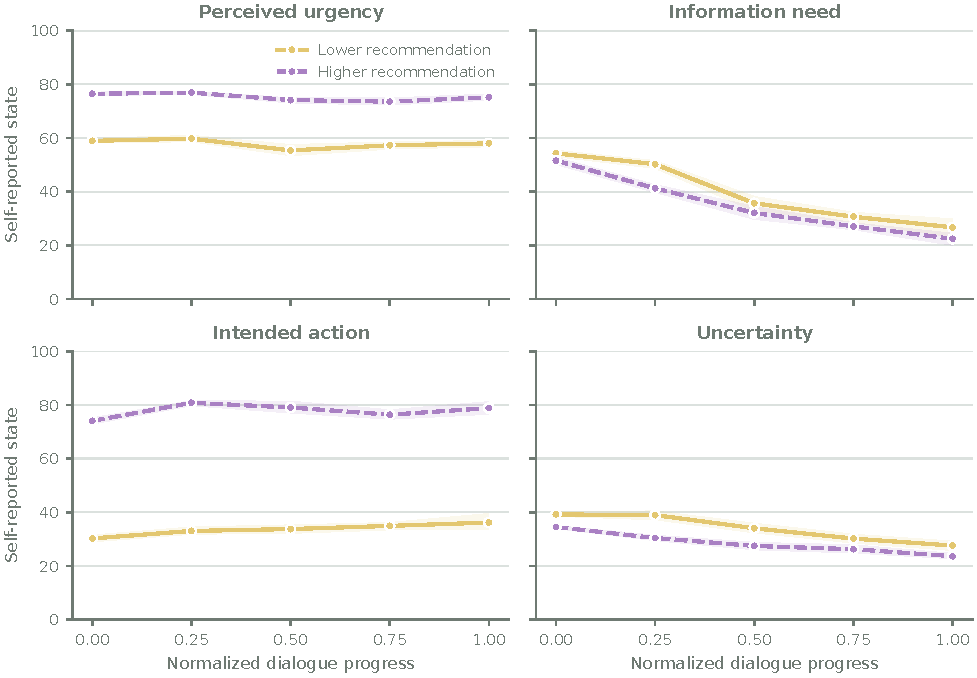
\includegraphics[width=\linewidth]{figs/v8_state_trajectories.pdf}
  \caption{Simulated-user self-reported-state trajectories. Means show how the four states evolve across completed dialogue cycles in the V8 transition dataset.}
  \label{fig:v8-trajectories}
\end{figure}

\begin{figure}[t]
  \centering
  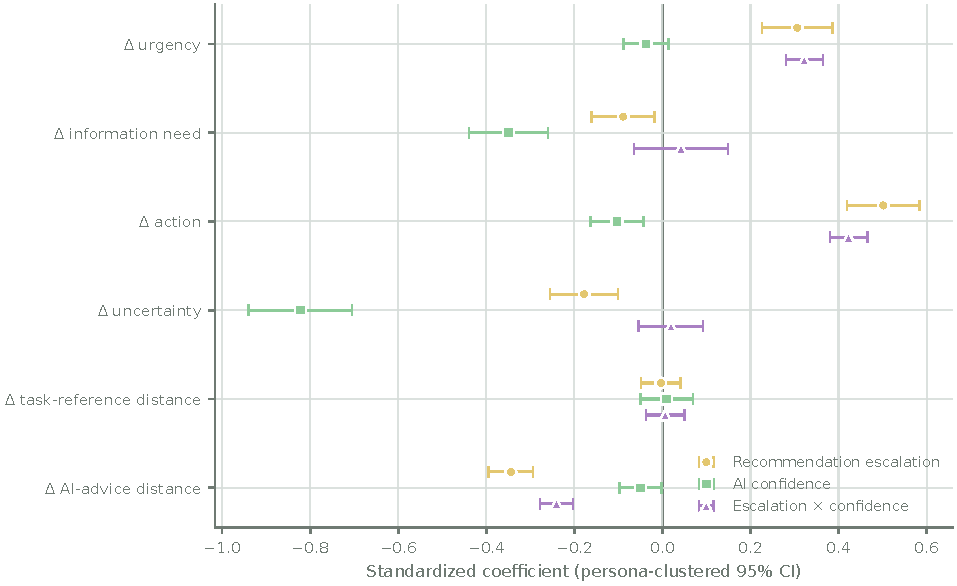
\includegraphics[width=\linewidth]{figs/v8_ai_influence_forest.pdf}
  \caption{Conditional transition coefficients. The forest plot reports standardized associations between experimental inputs and within-dialogue updating. Intervals use persona-clustered standard errors and should be interpreted with four persona clusters.}
  \label{fig:v8-forest}
\end{figure}

\begin{figure}[t]
  \centering
  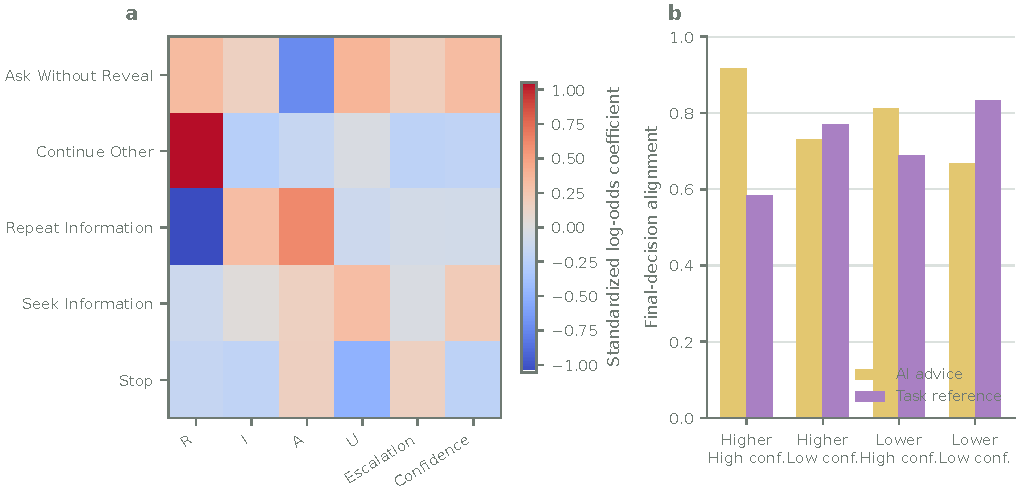
\includegraphics[width=\linewidth]{figs/v8_policy_and_final_decision.pdf}
  \caption{Advice responsiveness versus task-reference convergence. The panels distinguish movement toward the AI-advised endpoint from movement toward the fixed case reference.}
  \label{fig:v8-policy}
\end{figure}

\subsection{Human-freeze audit}

The main text reports the 109 completed participant records in the 2026-09-03 backup. They contain 218 completed case trajectories and 941 state ratings: 184 baseline and 757 post-turn reports. After chronological reindexing, 159 trajectories contain at least one post-turn probe. Qualtrics randomized the AI-assisted versus human-reasoning condition. Within AI-assisted sessions, recommendation level and AI confidence were balanced at session creation and fixed before interaction. A recommendation-bearing statement appeared in every returned assistant response, so delivered exposure required a participant message and response. Eighty-two case trajectories meet that exposure definition; 46 are viral-gastroenteritis trajectories forming the four-cell comparison (cell sizes 14, 11, 12, and 9 for lower/low, lower/high, higher/low, and higher/high). Recommendation analyses condition on delivered case-level exposure and are descriptive; delivered exposure itself was not independently randomized.

The raw UI payload counter restarted within otherwise continuous case histories. The analysis retains every rating, sorts events by timestamp, assigns baseline to turn 0, and renumbers post-turn ratings sequentially within participant and case. The original payload index is retained as \texttt{logged\_turn\_index} for audit. This prevents different chronological cycles from being collapsed into the same plotted turn. Human turn-level counts after correction are 159, 147, 142, 130, 93, 43, 20, 8, 5, 4, 3, 2, and 1 for turns 1--13 across cases; case-specific counts are reported in the reproducibility export.

Across the 82 recommendation-exposed trajectories, the median case-level mean assistant latency was 10.39 seconds (range 3.11--21.78; 432 responses). The question-mark metric is literal punctuation, not a semantic question-act classifier. It remains in the exported audit table but is not plotted as a substantive measure of information seeking.

\begin{figure}[t]
  \centering
  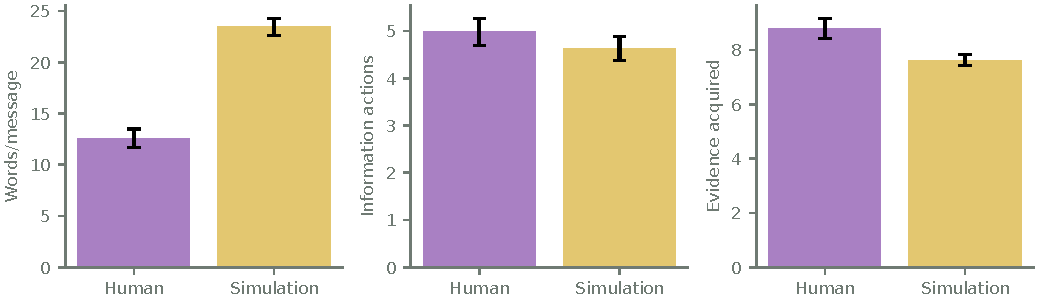
\includegraphics[width=\linewidth]{figs/human_simulation_conversation_comparison.pdf}
  \caption{Observable channels in matched viral gastroenteritis. Means and SEM across 46 recommendation-exposed human and 16 simulated trajectories. Message length differs substantially, while information actions and canonical evidence acquisition are closer in scale.}
  \label{fig:human-conversation}
\end{figure}

\subsection{Prespecified final-freeze human inference}

The final human analysis will fit context-only and context-plus-behavior ridge models using leave-one-participant-out prediction. The primary statistic is $\Delta R^2_{I,\mathrm{human}}$; the same statistic will be reported for urgency, action, and uncertainty. Information need is the prespecified confirmatory target, and the other states are secondary. Raw one-sided p-values and Holm--Bonferroni-adjusted p-values across all four states will be reported.

Because participant clusters have unequal trajectory lengths and cross-validated $\Delta R^2$ has no simple parametric null, inference will use participant-level randomization. Each permutation preserves a participant's context--probe pairs and reassigns complete behavioral sequences only among donors with the same case. Sequences are aligned chronologically; after a donor sequence stops, current-turn actions remain absent and cumulative evidence is carried forward. LOPO models will be refit for 5,000 Monte Carlo permutations (seed 20260812), with a plus-one-corrected one-sided p-value.

Magnitude uncertainty will use 5,000 participant-cluster bootstrap resamples (seed 20260813), sampling participants with all their eligible cases and turns and refitting the LOPO contrast. Percentile 95\% intervals will describe precision. These procedures will be run once at the final data freeze. Interim backups are used for descriptive trajectory and exposure audits only, which avoids optional stopping while recruitment is active.

\subsection{Reproducibility and release boundary}

Simulation code, task definitions, configuration, persona-grouped splits, analysis scripts, and derived nonhuman artifacts are prepared for public release. Human release materials contain only approved aggregated or de-identified fields and follow the consent and protocol restrictions. Private paths, credentials, SONA tokens, linkage secrets, and API keys are excluded. The analysis script preserves raw logged turn indices alongside corrected chronological indices, writes per-turn sample counts, and generates the manuscript figures from exported tables. The release URL is pending final repository publication.

\section*{NeurIPS Paper Checklist}

\begin{enumerate}

\item {\bf Claims}
    \item[] Question: Do the main claims made in the abstract and introduction accurately reflect the paper's contributions and scope?
    \item[] Answer: \answerYes{}
    \item[] Justification: The abstract and Introduction frame the main result as selective behavioral observability in persona agents. The 109-participant human sample provides descriptive matched comparisons; formal human behavioral-observability and participant-clustered transfer inference remain pending.
    \item[] Guidelines:
    \begin{itemize}
        \item The answer \answerNA{} means that the abstract and introduction do not include the claims made in the paper.
        \item The abstract and/or introduction should clearly state the claims made, including the contributions made in the paper and important assumptions and limitations. A \answerNo{} or \answerNA{} answer to this question will not be perceived well by the reviewers. 
        \item The claims made should match theoretical and experimental results, and reflect how much the results can be expected to generalize to other settings. 
        \item It is fine to include aspirational goals as motivation as long as it is clear that these goals are not attained by the paper. 
    \end{itemize}

\item {\bf Limitations}
    \item[] Question: Does the paper discuss the limitations of the work performed by the authors?
    \item[] Answer: \answerYes{}
    \item[] Justification: The Limitations and prospective test paragraph states the single-backbone, small-cohort, turn-cap, cross-domain, and expert-review limitations.
    \item[] Guidelines:
    \begin{itemize}
        \item The answer \answerNA{} means that the paper has no limitation while the answer \answerNo{} means that the paper has limitations, but those are not discussed in the paper. 
        \item The authors are encouraged to create a separate ``Limitations'' section in their paper.
        \item The paper should point out any strong assumptions and how robust the results are to violations of these assumptions (e.g., independence assumptions, noiseless settings, model well-specification, asymptotic approximations only holding locally). The authors should reflect on how these assumptions might be violated in practice and what the implications would be.
        \item The authors should reflect on the scope of the claims made, e.g., if the approach was only tested on a few datasets or with a few runs. In general, empirical results often depend on implicit assumptions, which should be articulated.
        \item The authors should reflect on the factors that influence the performance of the approach. For example, a facial recognition algorithm may perform poorly when image resolution is low or images are taken in low lighting. Or a speech-to-text system might not be used reliably to provide closed captions for online lectures because it fails to handle technical jargon.
        \item The authors should discuss the computational efficiency of the proposed algorithms and how they scale with dataset size.
        \item If applicable, the authors should discuss possible limitations of their approach to address problems of privacy and fairness.
        \item While the authors might fear that complete honesty about limitations might be used by reviewers as grounds for rejection, a worse outcome might be that reviewers discover limitations that aren't acknowledged in the paper. The authors should use their best judgment and recognize that individual actions in favor of transparency play an important role in developing norms that preserve the integrity of the community. Reviewers will be specifically instructed to not penalize honesty concerning limitations.
    \end{itemize}

\item {\bf Theory assumptions and proofs}
    \item[] Question: For each theoretical result, does the paper provide the full set of assumptions and a complete (and correct) proof?
    \item[] Answer: \answerNA{}
    \item[] Justification: The paper contains no theoretical results or proofs.
    \item[] Guidelines:
    \begin{itemize}
        \item The answer \answerNA{} means that the paper does not include theoretical results. 
        \item All the theorems, formulas, and proofs in the paper should be numbered and cross-referenced.
        \item All assumptions should be clearly stated or referenced in the statement of any theorems.
        \item The proofs can either appear in the main paper or the supplemental material, but if they appear in the supplemental material, the authors are encouraged to provide a short proof sketch to provide intuition. 
        \item Inversely, any informal proof provided in the core of the paper should be complemented by formal proofs provided in appendix or supplemental material.
        \item Theorems and Lemmas that the proof relies upon should be properly referenced. 
    \end{itemize}

    \item {\bf Experimental result reproducibility}
    \item[] Question: Does the paper fully disclose all the information needed to reproduce the main experimental results of the paper to the extent that it affects the main claims and/or conclusions of the paper (regardless of whether the code and data are provided or not)?
    \item[] Answer: \answerYes{}
    \item[] Justification: Sections 2--3 and the supplement report the agent backbone, pinned MatrAIx commit, cohort, cases, factorial conditions, probe schedules, grouped-persona evaluation, sample sizes, and exclusion of the invalid preliminary run.
    \item[] Guidelines:
    \begin{itemize}
        \item The answer \answerNA{} means that the paper does not include experiments.
        \item If the paper includes experiments, a \answerNo{} answer to this question will not be perceived well by the reviewers: Making the paper reproducible is important, regardless of whether the code and data are provided or not.
        \item If the contribution is a dataset and\slash or model, the authors should describe the steps taken to make their results reproducible or verifiable. 
        \item Depending on the contribution, reproducibility can be accomplished in various ways. For example, if the contribution is a novel architecture, describing the architecture fully might suffice, or if the contribution is a specific model and empirical evaluation, it may be necessary to either make it possible for others to replicate the model with the same dataset, or provide access to the model. In general. releasing code and data is often one good way to accomplish this, but reproducibility can also be provided via detailed instructions for how to replicate the results, access to a hosted model (e.g., in the case of a large language model), releasing of a model checkpoint, or other means that are appropriate to the research performed.
        \item While NeurIPS does not require releasing code, the conference does require all submissions to provide some reasonable avenue for reproducibility, which may depend on the nature of the contribution. For example
        \begin{enumerate}
            \item If the contribution is primarily a new algorithm, the paper should make it clear how to reproduce that algorithm.
            \item If the contribution is primarily a new model architecture, the paper should describe the architecture clearly and fully.
            \item If the contribution is a new model (e.g., a large language model), then there should either be a way to access this model for reproducing the results or a way to reproduce the model (e.g., with an open-source dataset or instructions for how to construct the dataset).
            \item We recognize that reproducibility may be tricky in some cases, in which case authors are welcome to describe the particular way they provide for reproducibility. In the case of closed-source models, it may be that access to the model is limited in some way (e.g., to registered users), but it should be possible for other researchers to have some path to reproducing or verifying the results.
        \end{enumerate}
    \end{itemize}


\item {\bf Open access to data and code}
    \item[] Question: Does the paper provide open access to the data and code, with sufficient instructions to faithfully reproduce the main experimental results, as described in supplemental material?
    \item[] Answer: \answerNo{}
    \item[] Justification: The figure-reproduction code, aggregate data, validation checks, and simulated-user artifacts are prepared in a documented repository, but the repository remains private pending final publication and license confirmation.
    \item[] Guidelines:
    \begin{itemize}
        \item The answer \answerNA{} means that paper does not include experiments requiring code.
        \item Please see the NeurIPS code and data submission guidelines (\url{https://neurips.cc/public/guides/CodeSubmissionPolicy}) for more details.
        \item While we encourage the release of code and data, we understand that this might not be possible, so \answerNo{} is an acceptable answer. Papers cannot be rejected simply for not including code, unless this is central to the contribution (e.g., for a new open-source benchmark).
        \item The instructions should contain the exact command and environment needed to run to reproduce the results. See the NeurIPS code and data submission guidelines (\url{https://neurips.cc/public/guides/CodeSubmissionPolicy}) for more details.
        \item The authors should provide instructions on data access and preparation, including how to access the raw data, preprocessed data, intermediate data, and generated data, etc.
        \item The authors should provide scripts to reproduce all experimental results for the new proposed method and baselines. If only a subset of experiments are reproducible, they should state which ones are omitted from the script and why.
        \item At submission time, to preserve anonymity, the authors should release anonymized versions (if applicable).
        \item Providing as much information as possible in supplemental material (appended to the paper) is recommended, but including URLs to data and code is permitted.
    \end{itemize}


\item {\bf Experimental setting/details}
    \item[] Question: Does the paper specify all the training and test details (e.g., data splits, hyperparameters, how they were chosen, type of optimizer) necessary to understand the results?
    \item[] Answer: \answerYes{}
    \item[] Justification: Section 2 specifies the 2-by-2 conditions, state probes, experimental context, regularized models, grouped-by-persona cross-validation, and trial/turn counts; the supplement gives additional design details.
    \item[] Guidelines:
    \begin{itemize}
        \item The answer \answerNA{} means that the paper does not include experiments.
        \item The experimental setting should be presented in the core of the paper to a level of detail that is necessary to appreciate the results and make sense of them.
        \item The full details can be provided either with the code, in appendix, or as supplemental material.
    \end{itemize}

\item {\bf Experiment statistical significance}
    \item[] Question: Does the paper report error bars suitably and correctly defined or other appropriate information about the statistical significance of the experiments?
    \item[] Answer: \answerNo{}
    \item[] Justification: The paper reports standard errors for trajectory and condition summaries, calculated across available participants or agent trials at each plotted turn or condition. Formal human transfer inference is reserved for the completed data freeze, when prespecified one-sided participant-level permutation tests and participant-cluster bootstrap intervals will be run. Four personas and one backbone do not support population-level inference about persona-agent effects or moderators.
    \item[] Guidelines:
    \begin{itemize}
        \item The answer \answerNA{} means that the paper does not include experiments.
        \item The authors should answer \answerYes{} if the results are accompanied by error bars, confidence intervals, or statistical significance tests, at least for the experiments that support the main claims of the paper.
        \item The factors of variability that the error bars are capturing should be clearly stated (for example, train/test split, initialization, random drawing of some parameter, or overall run with given experimental conditions).
        \item The method for calculating the error bars should be explained (closed form formula, call to a library function, bootstrap, etc.)
        \item The assumptions made should be given (e.g., Normally distributed errors).
        \item It should be clear whether the error bar is the standard deviation or the standard error of the mean.
        \item It is OK to report 1-sigma error bars, but one should state it. The authors should preferably report a 2-sigma error bar than state that they have a 96\% CI, if the hypothesis of Normality of errors is not verified.
        \item For asymmetric distributions, the authors should be careful not to show in tables or figures symmetric error bars that would yield results that are out of range (e.g., negative error rates).
        \item If error bars are reported in tables or plots, the authors should explain in the text how they were calculated and reference the corresponding figures or tables in the text.
    \end{itemize}

\item {\bf Experiments compute resources}
    \item[] Question: For each experiment, does the paper provide sufficient information on the computer resources (type of compute workers, memory, time of execution) needed to reproduce the experiments?
    \item[] Answer: \answerNo{}
    \item[] Justification: The manuscript identifies the GPT-4.1-mini backbone and trial count, but wall-clock time, API throughput, and hardware memory are not available as stable reproducibility quantities for the hosted-model run.
    \item[] Guidelines:
    \begin{itemize}
        \item The answer \answerNA{} means that the paper does not include experiments.
        \item The paper should indicate the type of compute workers CPU or GPU, internal cluster, or cloud provider, including relevant memory and storage.
        \item The paper should provide the amount of compute required for each of the individual experimental runs as well as estimate the total compute. 
        \item The paper should disclose whether the full research project required more compute than the experiments reported in the paper (e.g., preliminary or failed experiments that didn't make it into the paper). 
    \end{itemize}
    
\item {\bf Code of ethics}
    \item[] Question: Does the research conducted in the paper conform, in every respect, with the NeurIPS Code of Ethics \url{https://neurips.cc/public/EthicsGuidelines}?
    \item[] Answer: \answerYes{}
    \item[] Justification: The simulation and approved human study are reported with separate evidence status. The manuscript preserves participant anonymity and treats the 109-participant results as descriptive human--simulation comparisons pending the prespecified formal transfer analysis.
    \item[] Guidelines:
    \begin{itemize}
        \item The answer \answerNA{} means that the authors have not reviewed the NeurIPS Code of Ethics.
        \item If the authors answer \answerNo, they should explain the special circumstances that require a deviation from the Code of Ethics.
        \item The authors should make sure to preserve anonymity (e.g., if there is a special consideration due to laws or regulations in their jurisdiction).
    \end{itemize}


\item {\bf Broader impacts}
    \item[] Question: Does the paper discuss both potential positive societal impacts and negative societal impacts of the work performed?
    \item[] Answer: \answerYes{}
    \item[] Justification: The Introduction and Limitations discuss the benefit of testing simulation validity before recruitment and risks of flattening groups, model-specific relationships, and invalid transfer to people.
    \item[] Guidelines:
    \begin{itemize}
        \item The answer \answerNA{} means that there is no societal impact of the work performed.
        \item If the authors answer \answerNA{} or \answerNo, they should explain why their work has no societal impact or why the paper does not address societal impact.
        \item Examples of negative societal impacts include potential malicious or unintended uses (e.g., disinformation, generating fake profiles, surveillance), fairness considerations (e.g., deployment of technologies that could make decisions that unfairly impact specific groups), privacy considerations, and security considerations.
        \item The conference expects that many papers will be foundational research and not tied to particular applications, let alone deployments. However, if there is a direct path to any negative applications, the authors should point it out. For example, it is legitimate to point out that an improvement in the quality of generative models could be used to generate Deepfakes for disinformation. On the other hand, it is not needed to point out that a generic algorithm for optimizing neural networks could enable people to train models that generate Deepfakes faster.
        \item The authors should consider possible harms that could arise when the technology is being used as intended and functioning correctly, harms that could arise when the technology is being used as intended but gives incorrect results, and harms following from (intentional or unintentional) misuse of the technology.
        \item If there are negative societal impacts, the authors could also discuss possible mitigation strategies (e.g., gated release of models, providing defenses in addition to attacks, mechanisms for monitoring misuse, mechanisms to monitor how a system learns from feedback over time, improving the efficiency and accessibility of ML).
    \end{itemize}
    
\item {\bf Safeguards}
    \item[] Question: Does the paper describe safeguards that have been put in place for responsible release of data or models that have a high risk for misuse (e.g., pre-trained language models, image generators, or scraped datasets)?
    \item[] Answer: \answerNA{}
    \item[] Justification: The paper does not release a new foundation model, scraped dataset, or other high-risk asset requiring additional safeguards.
    \item[] Guidelines:
    \begin{itemize}
        \item The answer \answerNA{} means that the paper poses no such risks.
        \item Released models that have a high risk for misuse or dual-use should be released with necessary safeguards to allow for controlled use of the model, for example by requiring that users adhere to usage guidelines or restrictions to access the model or implementing safety filters. 
        \item Datasets that have been scraped from the Internet could pose safety risks. The authors should describe how they avoided releasing unsafe images.
        \item We recognize that providing effective safeguards is challenging, and many papers do not require this, but we encourage authors to take this into account and make a best faith effort.
    \end{itemize}

\item {\bf Licenses for existing assets}
    \item[] Question: Are the creators or original owners of assets (e.g., code, data, models), used in the paper, properly credited and are the license and terms of use explicitly mentioned and properly respected?
    \item[] Answer: \answerNo{}
    \item[] Justification: MatrAIx and the public administrative and regulatory sources are credited and versioned where applicable, but the release license and complete upstream asset-license inventory require final author confirmation before repository publication.
    \item[] Guidelines:
    \begin{itemize}
        \item The answer \answerNA{} means that the paper does not use existing assets.
        \item The authors should cite the original paper that produced the code package or dataset.
        \item The authors should state which version of the asset is used and, if possible, include a URL.
        \item The name of the license (e.g., CC-BY 4.0) should be included for each asset.
        \item For scraped data from a particular source (e.g., website), the copyright and terms of service of that source should be provided.
        \item If assets are released, the license, copyright information, and terms of use in the package should be provided. For popular datasets, \url{paperswithcode.com/datasets} has curated licenses for some datasets. Their licensing guide can help determine the license of a dataset.
        \item For existing datasets that are re-packaged, both the original license and the license of the derived asset (if it has changed) should be provided.
        \item If this information is not available online, the authors are encouraged to reach out to the asset's creators.
    \end{itemize}

\item {\bf New assets}
    \item[] Question: Are new assets introduced in the paper well documented and is the documentation provided alongside the assets?
    \item[] Answer: \answerNA{}
    \item[] Justification: No new public dataset or model is released with this submission. The prepared figure-reproduction package includes a README, dependency specifications, aggregate data documentation, scripts, outputs, and validation checks.
    \item[] Guidelines:
    \begin{itemize}
        \item The answer \answerNA{} means that the paper does not release new assets.
        \item Researchers should communicate the details of the dataset\slash code\slash model as part of their submissions via structured templates. This includes details about training, license, limitations, etc. 
        \item The paper should discuss whether and how consent was obtained from people whose asset is used.
        \item At submission time, remember to anonymize your assets (if applicable). You can either create an anonymized URL or include an anonymized zip file.
    \end{itemize}

\item {\bf Crowdsourcing and research with human subjects}
    \item[] Question: For crowdsourcing experiments and research with human subjects, does the paper include the full text of instructions given to participants and screenshots, if applicable, as well as details about compensation (if any)? 
    \item[] Answer: \answerNo{}
    \item[] Justification: The supplement reports the initial human sample, crossover structure, recorded measures, and exclusions, but the full participant instructions, interface screenshots, and compensation description are not yet included in this submission package.
    \item[] Guidelines:
    \begin{itemize}
        \item The answer \answerNA{} means that the paper does not involve crowdsourcing nor research with human subjects.
        \item Including this information in the supplemental material is fine, but if the main contribution of the paper involves human subjects, then as much detail as possible should be included in the main paper. 
        \item According to the NeurIPS Code of Ethics, workers involved in data collection, curation, or other labor should be paid at least the minimum wage in the country of the data collector. 
    \end{itemize}

\item {\bf Institutional review board (IRB) approvals or equivalent for research with human subjects}
    \item[] Question: Does the paper describe potential risks incurred by study participants, whether such risks were disclosed to the subjects, and whether Institutional Review Board (IRB) approvals (or an equivalent approval/review based on the requirements of your country or institution) were obtained?
    \item[] Answer: \answerYes{}
    \item[] Justification: The human study was conducted under Georgia Institute of Technology IRB protocol IRB2025-388 with informed consent, as stated in Section 4.1.
    \item[] Guidelines:
    \begin{itemize}
        \item The answer \answerNA{} means that the paper does not involve crowdsourcing nor research with human subjects.
        \item Depending on the country in which research is conducted, IRB approval (or equivalent) may be required for any human subjects research. If you obtained IRB approval, you should clearly state this in the paper. 
        \item We recognize that the procedures for this may vary significantly between institutions and locations, and we expect authors to adhere to the NeurIPS Code of Ethics and the guidelines for their institution. 
        \item For initial submissions, do not include any information that would break anonymity (if applicable), such as the institution conducting the review.
    \end{itemize}

\item {\bf Declaration of LLM usage}
    \item[] Question: Does the paper describe the usage of LLMs if it is an important, original, or non-standard component of the core methods in this research? Note that if the LLM is used only for writing, editing, or formatting purposes and does \emph{not} impact the core methodology, scientific rigor, or originality of the research, declaration is not required.
    %this research? 
    \item[] Answer: \answerYes{}
    \item[] Justification: Section 2 and the supplement disclose MatrAIx Persona-8B as the persona infrastructure, the pinned commit, GPT-4.1-mini as the persona-agent backbone, and the role of stateless self-report probes in the core methodology.
    \item[] Guidelines:
    \begin{itemize}
        \item The answer \answerNA{} means that the core method development in this research does not involve LLMs as any important, original, or non-standard components.
        \item Please refer to our LLM policy in the NeurIPS handbook for what should or should not be described.
    \end{itemize}

\end{enumerate}

\end{document}
